\documentclass[12pt,a4paper]{article}
\usepackage[utf8]{inputenc}
\usepackage[T1]{fontenc}
\usepackage[polish]{babel}
\usepackage{lmodern}
\usepackage{geometry}
\usepackage{graphicx}
\usepackage{float}
\usepackage{booktabs}
\usepackage{tabularx}
\usepackage{longtable}
\usepackage{array}
\usepackage{enumitem}
\usepackage{caption}
\usepackage{listings}
\usepackage{xcolor}
\usepackage{hyperref}
\usepackage{tikz}
\usepackage{pgfplots}
\pgfplotsset{compat=1.18}
\usetikzlibrary{arrows.meta,positioning,fit,calc,shapes.geometric,shapes.misc}

\geometry{margin=2.3cm}
\setlist[itemize]{leftmargin=1.5em}
\setlength{\parskip}{0.3em}
\setlength{\parindent}{0pt}

\lstdefinestyle{reportcode}{
  basicstyle=\ttfamily\small,
  breaklines=true,
  frame=single,
  backgroundcolor=\color{gray!5},
  columns=fullflexible
}

\hypersetup{
  colorlinks=true,
  linkcolor=blue!50!black,
  urlcolor=blue!50!black,
  pdftitle={Raport MVP - Behawioralna biometria ruchu myszy},
  pdfauthor={Piotr Kosiara, Emilia Anczarska}
}

\title{
  \textbf{Raport Techniczny MVP}\\
  \large Bot czy człowiek? Behawioralna biometria ruchu myszy\\
  dla ochrony aplikacji webowej
}
\author{Piotr Kosiara \\ Emilia Anczarska}
\date{\today}

\begin{document}

\maketitle
\tableofcontents
\newpage

\section{Wprowadzenie i motywacja}

\subsection{Kontekst problemu}
Aplikacje webowe są stale narażone na automatyczny ruch generowany przez boty:
masowe skanowanie zasobów, testowanie endpointów, tworzenie sztucznego ruchu
lub działania fraudowe. Klasyczne podejścia ochronne oparte wyłącznie o reguły
sieciowe i statyczne sygnatury przestają być wystarczające, ponieważ nowoczesne
boty potrafią imitować część zachowań użytkownika.

\subsection{Dlaczego behawioralna biometria myszy}
Trajektoria kursora, rytm kliknięć, dynamika scrollowania i przejścia focus/blur
niosą bogatą informację o sposobie interakcji człowieka z interfejsem.
W odróżnieniu od pojedynczego eventu, analiza krótkiego okna zachowania:

\begin{itemize}
  \item lepiej oddaje \textit{styl} interakcji,
  \item utrudnia prostym botom przejście niezauważonym,
  \item daje możliwość szybkiej reakcji ochronnej jeszcze w trakcie sesji.
\end{itemize}

\subsection{Cel projektu}
Celem MVP było zbudowanie kompletnego pipeline'u \textit{end-to-end}:
\begin{itemize}
  \item frontend zbiera telemetrykę zachowania i fingerprint środowiska,
  \item backend zapisuje sesje i surowe eventy,
  \item moduł cech buduje reprezentację okien zachowania,
  \item model klasyfikuje \texttt{human} vs \texttt{bot},
  \item silnik polityk zwraca akcję: \texttt{allow/observe/throttle/challenge/block}.
\end{itemize}

\subsection{Zakres i świadome uproszczenia MVP}
Wersja demonstracyjna została zaprojektowana profesjonalnie, ale celowo uproszczona:
\begin{itemize}
  \item inferencja modelu odbywa się w tym samym backendzie FastAPI (bez osobnego model service),
  \item predykcja działa na poziomie sesji i krótkich okien eventów,
  \item brak integracji z zewnętrznym WAF i blokadą IP (reakcja sesyjna),
  \item nacisk na czytelność kodu, odtwarzalność wyników i łatwą prezentację lokalną.
\end{itemize}

\section{Architektura systemu}

\subsection{Widok komponentów}
System składa się z czterech głównych części uruchamianych przez Docker Compose:
\begin{itemize}
  \item \textbf{Frontend} (Vite + React + TypeScript) -- zbiera telemetrię użytkownika.
  \item \textbf{Backend} (FastAPI) -- kolekcja eventów, predykcja, etykietowanie, API.
  \item \textbf{PostgreSQL} -- trwałe składowanie sesji, eventów, predykcji i akcji.
  \item \textbf{Bot Runner} (Playwright) -- generowanie powtarzalnych scenariuszy botowych.
\end{itemize}

\begin{figure}[H]
  \centering
  \resizebox{0.98\textwidth}{!}{\begin{tikzpicture}[
  x=1cm, y=1cm,
  comp/.style={
    rectangle,
    rounded corners,
    draw=black,
    very thick,
    align=center,
    text width=3.6cm,
    minimum height=1.3cm,
    fill=blue!6
  },
  store/.style={
    cylinder,
    shape border rotate=90,
    draw=black,
    very thick,
    align=center,
    text width=4.6cm,
    minimum height=1.8cm,
    aspect=0.27,
    fill=green!8
  },
  link/.style={-Latex, thick}
]

\node[comp, fill=orange!14] (user) at (0.0, 0.0) {Użytkownik\\(przeglądarka)};
\node[comp] (frontend) at (5.1, 0.0) {Frontend\\Vite + React};
\node[comp] (backend) at (10.6, 0.0) {Backend API\\FastAPI};
\node[store] (db) at (10.6, -3.1) {PostgreSQL\\sessions, events, predictions};
\node[comp, fill=purple!8] (bot) at (5.1, -2.4) {Bot Runner\\Playwright};
\node[comp, fill=teal!8] (ml) at (10.6, 3.2) {Feature Builder +\\Decision Tree + Policy};

\draw[link] (user) -- node[midway, above, fill=white, inner sep=1pt]{interakcje UI} (frontend);
\draw[link] (frontend) -- node[midway, above, fill=white, inner sep=1pt]{batch telemetry} (backend);
\draw[link] (backend) -- node[midway, right, fill=white, inner sep=1pt]{zapis/odczyt} (db);
\draw[link] (backend) -- node[midway, right, fill=white, inner sep=1pt]{okno cech i predykcja} (ml);
\draw[link, dashed] (bot) -- node[midway, left, fill=white, inner sep=1pt]{scenariusze botowe} (frontend);
\draw[link, dashed] (bot.east) to[bend left=14] node[midway, above, fill=white, inner sep=1pt]{etykietowanie botów} (backend.south west);

\end{tikzpicture}
}
  \caption{Architektura logiczna MVP}
\end{figure}

\subsection{Przepływ danych end-to-end}
\begin{enumerate}
  \item Frontend inicjuje sesję przez \texttt{POST /api/v1/sessions}.
  \item Kolektor telemetrii zbiera eventy i wysyła je batchami do \texttt{/api/v1/events/batch}.
  \item Backend zapisuje surowe dane do tabel \texttt{sessions} i \texttt{raw\_events}.
  \item Dla żądania predykcji backend buduje cechy z okna eventów.
  \item Model zwraca \texttt{predicted\_label}, prawdopodobieństwo bota i \texttt{risk\_score}.
  \item Policy engine mapuje \texttt{risk\_score} na akcję enforcement.
  \item Wynik i akcja są zapisywane (\texttt{predictions}, \texttt{enforcement\_actions}).
\end{enumerate}

\subsection{Diagram przypadków użycia}
\begin{figure}[H]
  \centering
  \resizebox{0.95\textwidth}{!}{\begin{tikzpicture}[
  x=1cm, y=1cm,
  actor/.style={draw, circle, minimum size=0.7cm, fill=gray!10},
  uc/.style={
    ellipse,
    draw=black,
    thick,
    align=center,
    minimum height=1.2cm,
    fill=blue!6,
    text width=6.4cm
  },
  line/.style={-Latex, thick}
]

\node[actor] (human) at (0.0,7.4) {};
\node[align=center] at (0.0,6.6) {Człowiek};

\node[actor] (bot) at (0.0,4.2) {};
\node[align=center] at (0.0,3.4) {Bot runner};

\node[actor] (operator) at (0.0,0.9) {};
\node[align=center] at (0.0,0.1) {Analityk};

\node[uc] (u1) at (8.2,7.4) {Generowanie\\telemetrii sesji};
\node[uc] (u2) at (8.2,5.8) {Wysłanie batcha eventów\\do Collector API};
\node[uc] (u3) at (8.2,4.2) {Predykcja human vs bot\\+ risk score};
\node[uc, text width=8.0cm] (u4) at (8.2,2.3) {Decyzja polityki\\allow/observe/throttle/challenge/block};
\node[uc] (u5) at (8.2,0.5) {Etykietowanie sesji\\do treningu};

\draw[line] (human) -- (u1);
\draw[line] (human) -- (u2);
\draw[line] (human) -- (u3);
\draw[line] (bot) -- (u1);
\draw[line] (bot) -- (u2);
\draw[line] (bot) -- (u3);
\draw[line] (operator) -- (u5);
\draw[line] (operator) -- (u4);

\draw[line, dashed] (u1.south) -- (u2.north);
\draw[line, dashed] (u2.south) -- (u3.north);
\draw[line, dashed] (u3.south) -- (u4.north);

\end{tikzpicture}
}
  \caption{Główne przypadki użycia systemu}
\end{figure}

\subsection{Model danych (ERD)}
\begin{figure}[H]
  \centering
  \resizebox{0.98\textwidth}{!}{\begin{tikzpicture}[
  x=1cm, y=1cm,
  tbl/.style={
    rectangle,
    draw=black,
    thick,
    align=left,
    font=\footnotesize,
    fill=green!6,
    text width=4.9cm,
    inner sep=5pt
  },
  rel/.style={-Latex, thick}
]

\node[tbl] (sessions) at (0.0, 4.8) {
\textbf{sessions}\\
PK: id\\
client\_fingerprint (JSON)\\
environment (JSON)\\
source, true\_label\\
started\_at\\
last\_event\_at
};

\node[tbl] (events) at (0.0, 1.0) {
\textbf{raw\_events}\\
PK: id\\
FK: session\_id $\rightarrow$ sessions.id\\
sequence\_no\\
event\_type, ts\_ms\\
x, y, scroll\_x, scroll\_y\\
target\_id, pointer\_type\\
payload
};

\node[tbl] (pred) at (7.0, 4.8) {
\textbf{predictions}\\
PK: id\\
FK: session\_id $\rightarrow$ sessions.id\\
FK: model\_version\_id $\rightarrow$ model\_versions.id\\
predicted\_label\\
probability\_bot\\
risk\_score, confidence\\
created\_at
};

\node[tbl] (modelv) at (7.0, 1.0) {
\textbf{model\_versions}\\
PK: id\\
name, version, algorithm\\
metrics (JSON)\\
artifact\_path\\
metadata (JSON)\\
created\_at
};

\node[tbl] (enf) at (7.0, -2.7) {
\textbf{enforcement\_actions}\\
PK: id\\
FK: session\_id $\rightarrow$ sessions.id\\
FK: prediction\_id $\rightarrow$ predictions.id\\
action, reason\\
created\_at
};

\draw[rel] (events.north) -- node[midway, left, fill=white, inner sep=1pt]{N:1} (sessions.south);
\draw[rel] (pred.west) -- node[midway, above, fill=white, inner sep=1pt]{N:1} (sessions.east);
\draw[rel] (pred.south) -- node[midway, right, fill=white, inner sep=1pt]{N:1} (modelv.north);
\draw[rel] (enf.north) -- node[midway, right, fill=white, inner sep=1pt]{N:1} (pred.south);
\draw[rel] (enf.west) to[bend right=24] node[pos=0.42, left, fill=white, inner sep=1pt]{N:1} (sessions.south east);

\end{tikzpicture}
}
  \caption{Relacyjny model danych PostgreSQL}
\end{figure}

\section{Dokumentacja techniczna codebase}

\subsection{Struktura repozytorium}
\begin{lstlisting}[style=reportcode]
Projekt_ADAC/
  backend/
    app/
      api/routes/            # endpointy FastAPI
      core/                  # konfiguracja, DB, logging
      models/                # ORM + schematy request/response
      repositories/          # dostep do danych
      services/              # feature engineering, policy, telemetry, trening danych
      ml/                    # trening i ewaluacja modelu
      scripts/               # seed i eksport replay
      tests/                 # testy jednostkowe
  frontend/
    src/
      api/                   # klient API
      components/            # testbed UI
      telemetry/             # collector + fingerprint + typy
  bot_runner/
    main.py                  # uruchamianie scenariuszy Playwright
    scenarios.py             # linear, human_like, adaptive, manual
  docker-compose.yml
  README.md
  raport/                    # dokumentacja LaTeX
\end{lstlisting}

\subsection{Frontend testbed (Vite + React + TypeScript)}
\subsubsection{Rola frontendu}
Frontend pelni podwojna funkcje:
\begin{itemize}
  \item \textbf{generatora naturalnych interakcji uzytkownika} (interfejs testowy),
  \item \textbf{sensora telemetrycznego} wysylajacego zdarzenia do backendu.
\end{itemize}

\subsubsection{Wyglad i funkcje interfejsu}
Widok frontendu pokazano na Rysunku~\ref{fig:frontend-ui}. Uklad ma trzy strefy:
\begin{itemize}
  \item \textbf{Panel sesji telemetrycznej} (gora): \texttt{session id}, liczniki eventow
  (\texttt{zbuforowane/wyslane}) i status collector pipeline.
  \item \textbf{Interaktywny testbed ruchu} (lewa kolumna): menu, wyszukiwarka,
  filtry kategorii, karty produktowe i przyciski CTA. To celowo przypomina
  realistyczny scenariusz e-commerce.
  \item \textbf{Silnik ochrony} (prawa kolumna): uruchamianie predykcji, reczne
  etykietowanie sesji (\texttt{human}/\texttt{bot}) i podglad wyniku:
  \texttt{risk score}, \texttt{predykcja}, \texttt{confidence}, \texttt{decyzja}.
\end{itemize}

\begin{figure}[H]
  \centering
  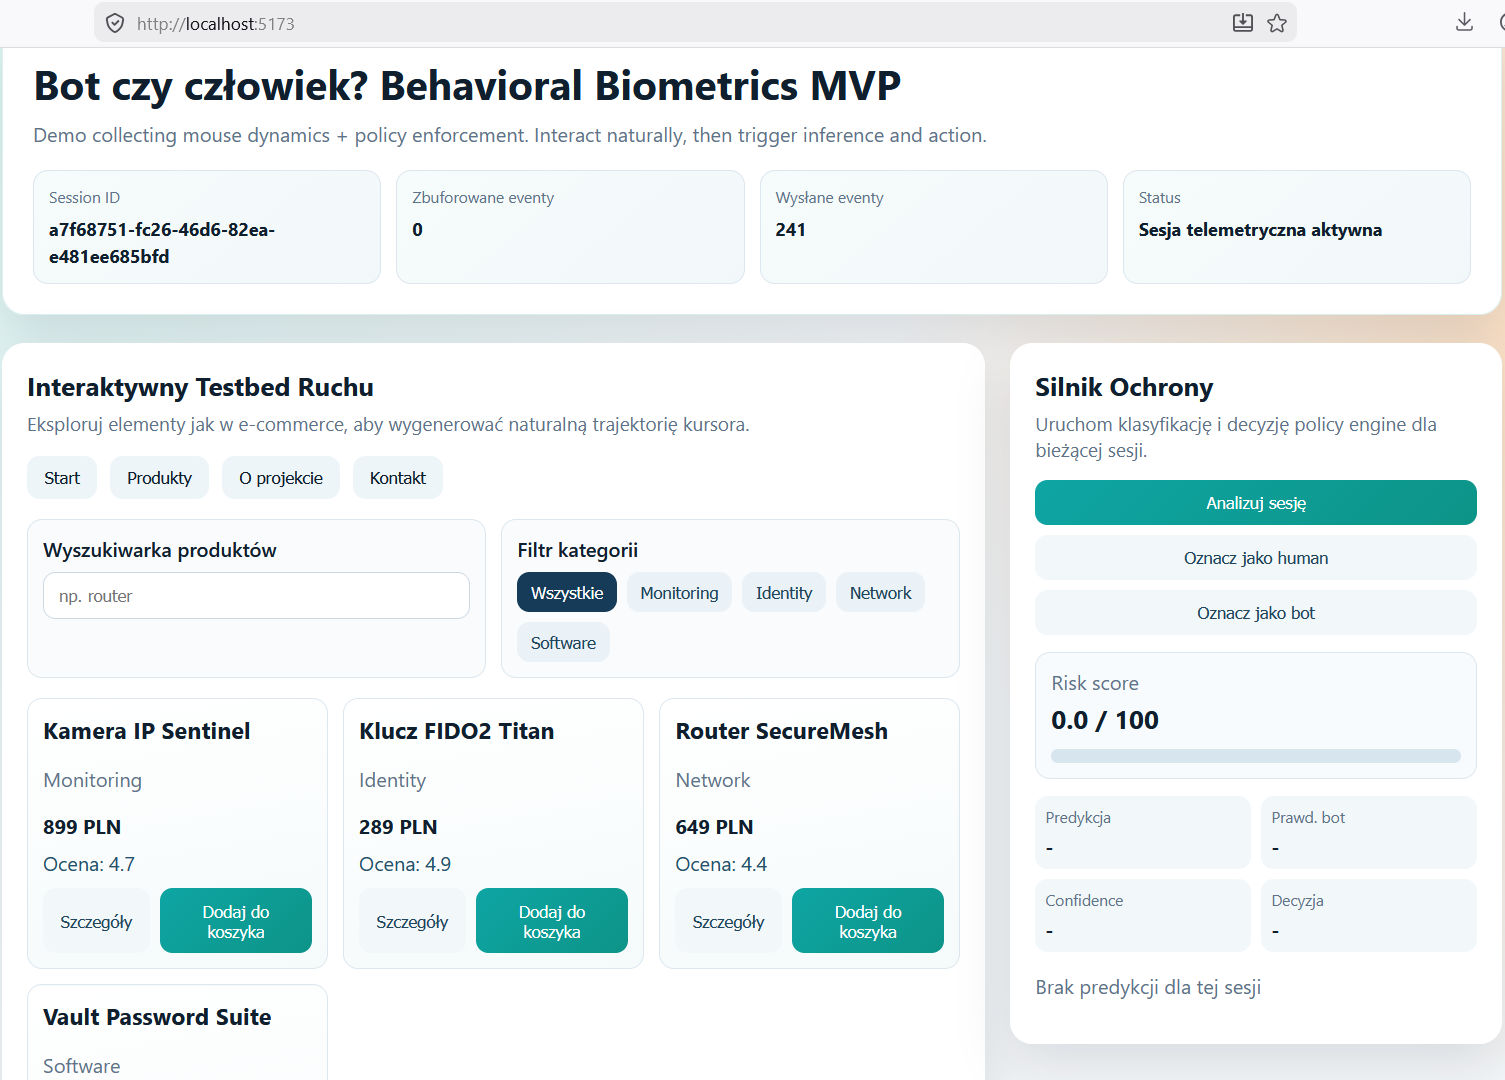
\includegraphics[width=0.98\textwidth]{frontend_view.png}
  \caption{Frontend testbed na localhost: panel telemetryczny, strefa interakcji i panel policy engine}
  \label{fig:frontend-ui}
\end{figure}

\subsubsection{Zbierane eventy i batching}
Kolektor (\texttt{frontend/src/telemetry/collector.ts}) rejestruje:
\begin{itemize}
  \item \texttt{mousemove},
  \item \texttt{click},
  \item \texttt{scroll},
  \item \texttt{focus},
  \item \texttt{blur},
  \item \texttt{viewport\_enter}/\texttt{viewport\_leave}
  (przez \texttt{visibilitychange}).
\end{itemize}

Wysylka odbywa sie partiami:
\begin{itemize}
  \item \texttt{batchSize = 35},
  \item okresowe \texttt{flush} co \texttt{2000 ms},
  \item retry: eventy wracaja do bufora przy bledzie API.
\end{itemize}

\subsubsection{Fingerprint klienta}
Zbierane cechy srodowiskowe obejmuja m.in.:
\begin{itemize}
  \item \texttt{user\_agent}, \texttt{language}, \texttt{timezone},
  \item \texttt{screen\_width/height}, \texttt{viewport\_width/height},
  \item \texttt{platform}, \texttt{pointer\_type},
  \item \texttt{webdriver}, \texttt{headless\_hint},
  \item \texttt{hardware\_concurrency}, \texttt{device\_memory}.
\end{itemize}

\subsection{Pozyskanie danych treningowych (human vs bot)}
\subsubsection{Jak zbierano dane klasy human}
Dane \texttt{human} byly zbierane manualnie przez interakcje operatora z frontendem
(Rysunek~\ref{fig:frontend-ui}): ruch myszy po menu, filtrach i kartach,
klikniecia, scrollowanie i wpisywanie fraz w wyszukiwarce.
Po zakonczonej probce sesje oznaczano przyciskiem \texttt{Oznacz jako human}.

\subsubsection{Jak zbierano dane klas botowych}
Sesje botowe generowano automatycznie przez \texttt{bot\_runner}:
\begin{lstlisting}[style=reportcode]
docker compose exec bot_runner python main.py --scenario linear --sessions 25 --record-video
docker compose exec bot_runner python main.py --scenario human_like --sessions 26 --record-video
docker compose exec bot_runner python main.py --scenario adaptive --sessions 50 --record-video
\end{lstlisting}

\subsubsection{Udzial scenariuszy botowych}
Na poziomie sesji botowych przyjeto:
\begin{itemize}
  \item \texttt{linear}: 25 sesji (24.75\% klasy bot),
  \item \texttt{human\_like}: 26 sesji (25.74\% klasy bot),
  \item \texttt{adaptive}: 50 sesji (49.50\% klasy bot).
\end{itemize}
Lacznie: 101 sesji botowych.

\subsubsection{Charakterystyka botow i zamysl projektowy}
\begin{itemize}
  \item \texttt{linear}: ruch prosty i rytmiczny, niski realizm.
  Cel: latwy baseline wykrywania prostych automatyzacji.
  \item \texttt{human\_like}: krzywe Beziera, jitter i losowe opoznienia.
  Cel: etap posredni pomiedzy botem prostym i trudniejszym.
  \item \texttt{adaptive}: scenariusz kalibrowany profilem zachowan czlowieka
  (\texttt{/api/v1/sessions/human-behavior-profile}), z dynamicznym tempem ruchu,
  pauzami, korektami toru i bardziej realistycznym typingiem.
  Cel: utrudnic klasyfikacje i przetestowac odpornosc modelu na boty
  zblizone dystrybucyjnie do klasy \texttt{human}.
\end{itemize}

\subsection{Backend Collector API (FastAPI)}
\subsubsection{Warstwy backendu}
\begin{itemize}
  \item \textbf{API routes} -- walidacja wejscia/wyjscia (Pydantic) i kontrakty REST.
  \item \textbf{Services} -- logika domenowa (telemetria, cechy, polityki, model).
  \item \textbf{Repositories} -- operacje bazodanowe (SQLAlchemy ORM).
  \item \textbf{ML module} -- trening i ewaluacja modelu.
\end{itemize}

\subsubsection{Endpointy REST}
\begin{longtable}{
  >{\ttfamily\footnotesize\raggedright\arraybackslash}p{0.47\textwidth}
  @{\hspace{1.0em}}
  >{\centering\arraybackslash}p{0.09\textwidth}
  @{\hspace{0.8em}}
  >{\raggedright\arraybackslash}p{0.32\textwidth}
}
\toprule
\textnormal{Endpoint} & \textnormal{Metoda} & \textnormal{Opis} \\
\midrule
\endhead
\textnormal{/api/v1/health} & GET & Healthcheck aplikacji. \\
\textnormal{/api/v1/sessions} & POST & Utworzenie nowej sesji i zapis fingerprintu. \\
\textnormal{/api/v1/events/batch} & POST & Przyjecie batcha eventow dla sesji. \\
\textnormal{/api/v1/sessions/\{session\_id\}/label} & POST & Etykietowanie sesji jako \texttt{human} lub \texttt{bot}. \\
\textnormal{/api/v1/predict/\{session\_id\}} & POST & Predykcja dla sesji + decyzja policy engine. \\
\textnormal{/api/v1/predictions/\{session\_id\}} & GET & Pobranie ostatniej predykcji sesji. \\
\textnormal{/api/v1/sessions/\{session\_id\}} & GET & Status sesji i metadane. \\
\textnormal{/api/v1/sessions/human-behavior-profile} & GET & Profil statystyczny zachowan czlowieka do adaptacji bota. \\
\bottomrule
\end{longtable}

\subsection{Storage: PostgreSQL}
Model danych sklada sie z pieciu tabel:
\begin{itemize}
  \item \texttt{sessions} -- glowna encja sesji,
  \item \texttt{raw\_events} -- surowy strumien interakcji,
  \item \texttt{predictions} -- wyniki modelu,
  \item \texttt{model\_versions} -- rejestr wersji modelu i metryk,
  \item \texttt{enforcement\_actions} -- decyzje polityki ochronnej.
\end{itemize}

Relacje opisuje diagram ERD w Sekcji 2.

\subsection{Slownik zmiennych bazodanowych}
Tabela~\ref{tab:db-variable-dictionary} pokazuje wszystkie zmienne przechowywane
w bazie PostgreSQL. Kolumna \texttt{czy wchodzi do modelu} oznacza, czy dana
zmienna jest wykorzystywana w pipeline cech (bezposrednio lub przez transformacje).

\begin{longtable}{
  >{\ttfamily\scriptsize\raggedright\arraybackslash\hspace{0pt}}p{0.33\textwidth}
  @{\hspace{1.0em}}
  >{\footnotesize\raggedright\arraybackslash}p{0.52\textwidth}
  @{\hspace{0.8em}}
  >{\footnotesize\centering\arraybackslash}p{0.06\textwidth}
}
\caption{Slownik zmiennych bazodanowych: znaczenie i udzial w modelu}
\label{tab:db-variable-dictionary} \\
\toprule
\textnormal{nazwa\_zmiennej} & \textnormal{co zmienna oznacza (jak jest wyliczana)} & \textnormal{czy wchodzi do modelu} \\
\midrule
\endfirsthead
\toprule
\textnormal{nazwa\_zmiennej} & \textnormal{co zmienna oznacza (jak jest wyliczana)} & \textnormal{czy wchodzi do modelu} \\
\midrule
\endhead
\textnormal{sessions.id} & identyfikator sesji (UUID). & NIE \\
\textnormal{sessions.source} & zrodlo sesji (np. \texttt{frontend} / \texttt{bot\_runner}). & NIE \\
\textnormal{sessions.true\_label} & etykieta referencyjna \texttt{human}/\texttt{bot} nadawana recznie lub automatycznie. & NIE \\
\textnormal{sessions.status} & status procesu sesji (np. collecting, predicted). & NIE \\
\textnormal{sessions.client\_fingerprint} & surowy fingerprint klienta (JSON). & NIE \\
\textnormal{sessions.environment} & surowe parametry srodowiskowe (JSON), zrodlo cech srodowiskowych. & TAK \\
\textnormal{sessions.created\_at} & czas utworzenia rekordu sesji. & NIE \\
\textnormal{sessions.updated\_at} & czas ostatniej aktualizacji sesji. & NIE \\
\textnormal{sessions.environment.user\_agent} & identyfikator przegladarki/OS; uzywany do flag pomocniczych. & TAK \\
\textnormal{sessions.environment.language} & jezyk przegladarki. & NIE \\
\textnormal{sessions.environment.timezone} & strefa czasowa klienta. & NIE \\
\textnormal{sessions.environment.screen\_width} & szerokosc ekranu klienta; skladnik \texttt{screen\_area}. & TAK \\
\textnormal{sessions.environment.screen\_height} & wysokosc ekranu klienta; skladnik \texttt{screen\_area}. & TAK \\
\textnormal{sessions.environment.viewport\_width} & szerokosc viewportu; skladnik \texttt{viewport\_area}. & TAK \\
\textnormal{sessions.environment.viewport\_height} & wysokosc viewportu; skladnik \texttt{viewport\_area}. & TAK \\
\textnormal{sessions.environment.webdriver} & flaga automatyzacji przegladarki. & TAK \\
\textnormal{sessions.environment.headless\_hint} & sygnal trybu headless. & TAK \\
\textnormal{sessions.environment.hardware\_concurrency} & liczba logicznych rdzeni CPU raportowana przez przegladarke. & TAK \\
\textnormal{sessions.environment.device\_memory} & pamiec urzadzenia raportowana przez przegladarke. & TAK \\
\textnormal{raw\_events.id} & techniczny identyfikator eventu. & NIE \\
\textnormal{raw\_events.session\_id} & klucz obcy do sesji. & NIE \\
\textnormal{raw\_events.sequence\_no} & numer sekwencyjny eventu w batchu. & NIE \\
\textnormal{raw\_events.event\_type} & typ eventu (\texttt{mousemove}, \texttt{click}, \texttt{scroll}, ...). & TAK \\
\textnormal{raw\_events.ts\_ms} & timestamp eventu w milisekundach, baza do dynamiki. & TAK \\
\textnormal{raw\_events.x} & pozycja X kursora. & TAK \\
\textnormal{raw\_events.y} & pozycja Y kursora. & TAK \\
\textnormal{raw\_events.scroll\_x} & przesuniecie poziome scrolla. & NIE \\
\textnormal{raw\_events.scroll\_y} & przesuniecie pionowe scrolla, baza \texttt{scroll\_velocity}. & TAK \\
\textnormal{raw\_events.target\_id} & identyfikator celu eventu; baza \texttt{hover/target\_revisit}. & TAK \\
\textnormal{raw\_events.target\_tag} & tag HTML celu interakcji. & NIE \\
\textnormal{raw\_events.target\_class} & klasy CSS celu interakcji. & NIE \\
\textnormal{raw\_events.pointer\_type} & typ urzadzenia wskazujacego. & NIE \\
\textnormal{raw\_events.in\_viewport} & flaga widocznosci eventu w viewport. & NIE \\
\textnormal{raw\_events.payload} & dodatkowy payload zdarzenia (JSON). & NIE \\
\textnormal{raw\_events.created\_at} & czas zapisu eventu. & NIE \\
\textnormal{predictions.id} & identyfikator predykcji. & NIE \\
\textnormal{predictions.session\_id} & sesja, dla ktorej wykonano predykcje. & NIE \\
\textnormal{predictions.model\_version\_id} & wersja modelu uzyta do inferencji. & NIE \\
\textnormal{predictions.predicted\_label} & wynik klasyfikacji modelu (\texttt{human}/\texttt{bot}). & NIE \\
\textnormal{predictions.probability\_bot} & prawdopodobienstwo klasy \texttt{bot}. & NIE \\
\textnormal{predictions.confidence} & pewnosc predykcji (maksimum prawdopodobienstwa). & NIE \\
\textnormal{predictions.risk\_score} & przeskalowany wynik ryzyka 0--100. & NIE \\
\textnormal{predictions.feature\_snapshot} & snapshot wektora cech wykorzystanych przy predykcji. & NIE \\
\textnormal{predictions.created\_at} & czas utworzenia predykcji. & NIE \\
\textnormal{model\_versions.id} & identyfikator wersji modelu. & NIE \\
\textnormal{model\_versions.name} & nazwa modelu. & NIE \\
\textnormal{model\_versions.version} & oznaczenie wersji (np. timestamp). & NIE \\
\textnormal{model\_versions.algorithm} & algorytm (Decision Tree). & NIE \\
\textnormal{model\_versions.feature\_set\_version} & wersja zestawu cech. & NIE \\
\textnormal{model\_versions.metrics} & metryki treningowe/ewaluacyjne (JSON). & NIE \\
\textnormal{model\_versions.artifact\_path} & sciezka do artefaktu modelu. & NIE \\
\textnormal{model\_versions.model\_metadata} & metadane modelu (JSON). & NIE \\
\textnormal{model\_versions.is\_active} & flaga aktywnej wersji modelu. & NIE \\
\textnormal{model\_versions.created\_at} & czas rejestracji wersji modelu. & NIE \\
\textnormal{enforcement\_actions.id} & identyfikator decyzji polityki. & NIE \\
\textnormal{enforcement\_actions.session\_id} & sesja, ktorej dotyczy decyzja. & NIE \\
\textnormal{enforcement\_actions.prediction\_id} & predykcja powiazana z decyzja. & NIE \\
\textnormal{enforcement\_actions.action} & decyzja (\texttt{allow}/\texttt{observe}/\texttt{throttle}/\texttt{challenge}/\texttt{block}). & NIE \\
\textnormal{enforcement\_actions.reason} & uzasadnienie decyzji polityki. & NIE \\
\textnormal{enforcement\_actions.blocked\_until} & koniec blokady czasowej (jesli dotyczy). & NIE \\
\textnormal{enforcement\_actions.action\_metadata} & dodatkowe metadane decyzji (JSON). & NIE \\
\textnormal{enforcement\_actions.created\_at} & czas zapisu decyzji. & NIE \\
\bottomrule
\end{longtable}

\subsection{Feature engineering}
Pipeline cech (\texttt{backend/app/services/feature\_engineering.py}) liczy cechy
z okna eventow posortowanych po czasie (\texttt{ts\_ms}), a nie z pojedynczego eventu.

\subsubsection{Przykladowe cechy dynamiczne}
\begin{itemize}
  \item trajektoria i geometria: \texttt{path\_length}, \texttt{displacement}, \texttt{path\_efficiency},
  \item dynamika ruchu: \texttt{speed\_mean/std/max}, \texttt{acc\_mean/std/max}, \texttt{jerk\_mean/std/max},
  \item mikrozachowania: \texttt{micro\_pause\_count}, \texttt{correction\_rhythm}, \texttt{overshoot\_count},
  \item klikniecia: \texttt{click\_interval\_mean/std}, \texttt{hover\_before\_click\_mean}, \texttt{target\_revisit\_count},
  \item kontekst sekwencji: \texttt{event\_type\_entropy}, \texttt{unique\_event\_types},
  \item scroll i focus: \texttt{scroll\_velocity\_mean/std}, \texttt{focus\_blur\_transitions}.
\end{itemize}

\subsubsection{Cechy srodowiskowe}
Pipeline zawiera takze cechy srodowiskowe, jednak w finalnym modelu drzewa
sa one \textbf{domyslnie wylaczone z treningu} (\texttt{feature\_set=behavioral}),
aby ograniczyc ryzyko data leakage (np. trywialny podzial po \texttt{viewport\_area}).

\subsubsection{Slownik zmiennych cechowych}
Tabela~\ref{tab:feature-dictionary} zawiera komplet zmiennych cechowych budowanych
w pipeline i informacje, czy dana zmienna wchodzi do finalnego modelu.

\begin{longtable}{
  >{\ttfamily\scriptsize\raggedright\arraybackslash\hspace{0pt}}p{0.27\textwidth}
  @{\hspace{1.0em}}
  >{\footnotesize\raggedright\arraybackslash}p{0.57\textwidth}
  @{\hspace{0.8em}}
  >{\footnotesize\centering\arraybackslash}p{0.06\textwidth}
}
\caption{Slownik zmiennych cechowych: nazwa, znaczenie i uzycie w modelu finalnym}
\label{tab:feature-dictionary} \\
\toprule
\textnormal{nazwa\_zmiennej} & \textnormal{co zmienna oznacza (jak jest wyliczana)} & \textnormal{czy wchodzi do modelu} \\
\midrule
\endfirsthead
\toprule
\textnormal{nazwa\_zmiennej} & \textnormal{co zmienna oznacza (jak jest wyliczana)} & \textnormal{czy wchodzi do modelu} \\
\midrule
\endhead
\textnormal{event\_count} & liczba wszystkich eventow w oknie czasowym. & TAK \\
\textnormal{window\_duration\_ms} & czas trwania okna: \texttt{ts\_last - ts\_first}. & TAK \\
\textnormal{mousemove\_count} & liczba eventow \texttt{mousemove}. & TAK \\
\textnormal{click\_count} & liczba eventow \texttt{click}. & TAK \\
\textnormal{scroll\_count} & liczba eventow \texttt{scroll}. & TAK \\
\textnormal{focus\_blur\_transitions} & suma liczby eventow \texttt{focus} i \texttt{blur}. & TAK \\
\textnormal{viewport\_enter\_count} & liczba eventow \texttt{viewport\_enter}. & TAK \\
\textnormal{viewport\_leave\_count} & liczba eventow \texttt{viewport\_leave}. & TAK \\
\textnormal{path\_length} & suma odleglosci euklidesowych pomiedzy kolejnymi punktami kursora. & TAK \\
\textnormal{displacement} & odleglosc miedzy pierwszym i ostatnim punktem kursora w oknie. & TAK \\
\textnormal{path\_efficiency} & wspolczynnik \texttt{displacement / max(path\_length, 1)}. & TAK \\
\textnormal{speed\_mean} & srednia predkosc kursora pomiedzy kolejnymi punktami (\texttt{distance/dt}). & TAK \\
\textnormal{speed\_std} & odchylenie standardowe predkosci kursora. & TAK \\
\textnormal{speed\_max} & maksymalna predkosc kursora w oknie. & TAK \\
\textnormal{acc\_mean} & srednie przyspieszenie: \texttt{delta(speed)/dt}. & TAK \\
\textnormal{acc\_std} & odchylenie standardowe przyspieszenia. & TAK \\
\textnormal{acc\_max} & maksymalne przyspieszenie w oknie. & TAK \\
\textnormal{jerk\_mean} & sredni jerk: \texttt{delta(acc)/dt}. & TAK \\
\textnormal{jerk\_std} & odchylenie standardowe jerk. & TAK \\
\textnormal{jerk\_max} & maksymalny jerk w oknie. & TAK \\
\textnormal{curvature\_mean} & srednia krzywizna toru: \texttt{|delta(kat)| / max(distance, 1)}. & TAK \\
\textnormal{curvature\_std} & odchylenie standardowe krzywizny toru. & TAK \\
\textnormal{angle\_change\_mean} & srednia zmiana kata ruchu pomiedzy kolejnymi segmentami. & TAK \\
\textnormal{angle\_change\_std} & odchylenie standardowe zmian kata ruchu. & TAK \\
\textnormal{micro\_pause\_count} & liczba segmentow z bardzo niska predkoscia (\texttt{speed < 40 px/s}). & TAK \\
\textnormal{correction\_rhythm} & liczba mocnych korekt kierunku (prog zmiany kata \texttt{> 1.1 rad}). & TAK \\
\textnormal{click\_interval\_mean} & sredni odstep czasowy miedzy kolejnymi kliknieciami. & TAK \\
\textnormal{click\_interval\_std} & odchylenie standardowe odstepow miedzy kliknieciami. & TAK \\
\textnormal{hover\_before\_click\_mean} & sredni czas hover przed kliknieciem, liczony lokalnie przy celu klikniecia. & TAK \\
\textnormal{dwell\_time\_mean} & sredni czas przebywania na segmentach (\texttt{1000/max(speed,1)}). & TAK \\
\textnormal{overshoot\_count} & liczba przypadkow overshoot (rewersy kierunku przed kliknieciem). & TAK \\
\textnormal{target\_revisit\_count} & liczba celow klikanych wielokrotnie w tej samej sesji okna. & TAK \\
\textnormal{scroll\_velocity\_mean} & srednia predkosc scrolla: \texttt{|delta(scroll\_y)|/dt}. & TAK \\
\textnormal{scroll\_velocity\_std} & odchylenie standardowe predkosci scrolla. & TAK \\
\textnormal{unique\_event\_types} & liczba unikalnych typow eventow w oknie. & TAK \\
\textnormal{event\_type\_entropy} & entropia Shannona rozkladu typow eventow w oknie. & TAK \\
\textnormal{webdriver\_flag} & flaga 0/1: czy \texttt{navigator.webdriver} jest prawda. & NIE \\
\textnormal{headless\_flag} & flaga 0/1: wykrycie sygnalu headless na podstawie \texttt{user-agent}. & NIE \\
\textnormal{viewport\_area} & pole viewportu: \texttt{viewport\_width * viewport\_height}. & NIE \\
\textnormal{screen\_area} & pole ekranu: \texttt{screen\_width * screen\_height}. & NIE \\
\textnormal{viewport\_screen\_ratio} & iloraz \texttt{viewport\_area / max(screen\_area,1)}. & NIE \\
\textnormal{hardware\_concurrency} & liczba logicznych rdzeni CPU raportowana przez przegladarke. & NIE \\
\textnormal{device\_memory} & pamiec urzadzenia raportowana przez przegladarke. & NIE \\
\bottomrule
\end{longtable}

\subsection{Model i inferencja}
\subsubsection{Trening offline}
Skrypt \texttt{python -m app.ml.train} realizuje:
\begin{itemize}
  \item budowe DataFrame z okien (\texttt{window\_size}, \texttt{stride}),
  \item podzial train/test z grupowaniem po \texttt{session\_id} (\texttt{GroupShuffleSplit}),
  \item trening \texttt{DecisionTreeClassifier} z \texttt{class\_weight=balanced},
  \item zapis artefaktow: model, metryki, ROC, confusion matrix, drzewo i reguly.
\end{itemize}

\subsubsection{Predykcja online}
Inferencja dziala przez \texttt{ModelManager}:
\begin{itemize}
  \item laduje aktywny artefakt modelu (\texttt{active\_model.joblib}),
  \item zwraca \texttt{predicted\_label}, \texttt{probability\_bot}, \texttt{confidence}, \texttt{risk\_score},
  \item przy braku modelu uzywa fallbacku heurystycznego.
\end{itemize}

\subsection{Policy engine / enforcement}
Mapowanie ryzyka (\texttt{backend/app/services/policy\_engine.py}):
\begin{itemize}
  \item \texttt{risk < 25}: \texttt{allow},
  \item \texttt{25--50}: \texttt{observe},
  \item \texttt{50--75}: \texttt{throttle},
  \item \texttt{75--90}: \texttt{challenge},
  \item \texttt{>= 90}: \texttt{block}.
\end{itemize}

\subsection{DevOps i uruchomienie}
Srodowisko dziala lokalnie przez Docker Compose:
\begin{itemize}
  \item \texttt{frontend} -- port 5173,
  \item \texttt{backend} -- port 8000,
  \item \texttt{db} -- port 5432,
  \item \texttt{bot\_runner} -- kontener narzedziowy do generacji sesji.
\end{itemize}

\subsection{Jakosc i testy}
\begin{itemize}
  \item testy jednostkowe backendu (\texttt{backend/app/tests}),
  \item walidacja kontraktow API przez schematy Pydantic,
  \item separacja odpowiedzialnosci: API/Services/Repositories/ML.
\end{itemize}


\section{Model finalny i raport wynikow}

\subsection{Cel i zakres analizy modelu}
W tej sekcji dokumentujemy finalny model klasyfikacji \texttt{human} vs \texttt{bot},
z naciskiem na:
\begin{itemize}
  \item jakie dane i cechy weszly do treningu,
  \item jak wykonano podzial na trening i test,
  \item jak przeprowadzono walidacje i ewaluacje,
  \item na ile wyniki odpowiadaja rzeczywistemu dzialaniu systemu.
\end{itemize}

\subsection{Konfiguracja modelu finalnego}
Finalna wersja modelu to drzewo decyzyjne trenowane na cechach behawioralnych:
\begin{itemize}
  \item algorytm: \texttt{DecisionTreeClassifier},
  \item parametry okna: \texttt{window\_size = 120}, \texttt{stride = 80},
  \item hiperparametry: \texttt{max\_depth = 12}, \texttt{min\_samples\_leaf = 2},
  \item \texttt{class\_weight = balanced},
  \item \texttt{feature\_set = behavioral} (bez cech srodowiskowych).
\end{itemize}

\subsection{Jakie dane weszly do modelu}
\subsubsection{Poziom surowy}
Wejsciem sa sesje zapisane w PostgreSQL (\texttt{sessions}, \texttt{raw\_events}),
z etykieta referencyjna \texttt{true\_label} nadana przez operatora.
Kazde okno zawiera uporzadkowany po czasie fragment zachowania, a nie pojedynczy event.

\subsubsection{Poziom cech}
Z okna eventow budowane sa cechy opisujace:
\begin{itemize}
  \item dynamike ruchu kursora: \texttt{speed\_*}, \texttt{acc\_*}, \texttt{jerk\_*},
  \item geometrie toru: \texttt{path\_length}, \texttt{path\_efficiency}, \texttt{curvature\_*},
  \item mikrozachowania: \texttt{micro\_pause\_count}, \texttt{correction\_rhythm}, \texttt{overshoot\_count},
  \item wzorzec klikniec i scrolla: \texttt{click\_interval\_*}, \texttt{hover\_before\_click\_mean},
  \texttt{scroll\_velocity\_*},
  \item entropie sekwencji: \texttt{event\_type\_entropy}, \texttt{unique\_event\_types}.
\end{itemize}

W finalnym modelu swiadomie pominieto cechy srodowiskowe (np. \texttt{viewport\_area}),
zeby ograniczyc ryzyko sztucznego zawyzania wyniku przez data leakage.

\subsection{Dobor zmiennych: proces i uzasadnienie}
\subsubsection{Przestrzen kandydacka i finalny wybor}
Proces startowal od pelnego slownika cech wyliczanego przez pipeline
(\texttt{FEATURE\_COLUMNS}) opisany w Tabeli~\ref{tab:feature-dictionary}.
W praktyce byly to:
\begin{itemize}
  \item 43 cechy kandydackie lacznie,
  \item 7 cech srodowiskowych,
  \item 36 cech behawioralnych.
\end{itemize}

Do finalnego modelu weszly cechy behawioralne
(\texttt{feature\_set=behavioral}), natomiast cechy srodowiskowe zostaly
wylaczone z trenowania drzewa.

\subsubsection{Kryteria doboru zmiennych}
Selekcja byla oparta o trzy kryteria:
\begin{itemize}
  \item \textbf{odpornosc na leakage}: odciecie sygnalow typu
  \texttt{viewport\_area} i \texttt{screen\_area}, ktore moga rozdzielac klasy
  na skroty, bez realnej analizy zachowania,
  \item \textbf{zwiazek z mikrodynamika ruchu}: preferencja dla cech opisujacych
  kinetyke i geometrie toru (\texttt{acc\_*}, \texttt{speed\_*}, \texttt{curvature\_*}),
  \item \textbf{interpretowalnosc}: drzewo z tak dobranym zbiorem cech daje
  reguly decyzyjne, ktore mozna odczytac i wyjasnic.
\end{itemize}

\subsubsection{Co oznacza ten wybor w praktyce}
Model finalny klasyfikuje sesje glownie na podstawie \emph{jak} porusza sie kursor
i jak wyglada rytm interakcji, a nie \emph{na czym} sesja jest wykonywana.
To zwieksza wiarygodnosc demonstracji, bo decyzja nie wynika z jednego artefaktu
srodowiskowego, tylko z profilu zachowania.

\subsection{Podzial train/test i walidacja}
\subsubsection{Strategia podzialu}
Podzial zostal wykonany przez \texttt{GroupShuffleSplit} z \texttt{test\_size=0.25}
i grupowaniem po \texttt{session\_id}. To kluczowe, bo:
\begin{itemize}
  \item okna z tej samej sesji nie trafiaja jednoczesnie do train i test,
  \item test sprawdza uogolnienie na nieznane sesje, a nie tylko nieznane okna.
\end{itemize}

\subsubsection{Co oznaczaja liczby w praktyce}
Z raportu metryk treningowych (Tabela~\ref{tab:train-metrics} i
Tabela~\ref{tab:train-cm}) wynika, ze zbior testowy mial 136 okien
(\texttt{TN+FP+FN+TP = 74+1+6+55}).
W ewaluacji aktywnego modelu analizowano 644 okna i 202 sesje
(Tabela~\ref{tab:eval-operational}).

\subsubsection{Typ walidacji}
W MVP uzyto pojedynczego hold-out splitu grupowego (jedna probka walidacyjna).
To dobre rozwiazanie demonstracyjne, ale nie zastepuje pelnej walidacji krzyzowej
np. \texttt{GroupKFold}.

\subsection{Metryki ilosciowe}
% Auto-generated by raport/scripts/refresh_model_assets.ps1
% Source timestamp: 20260515_173306

\subsubsection{Metryki z treningu (hold-out, GroupShuffleSplit)}
\begin{table}[H]
  \centering
  \begin{tabular}{l c}
    \toprule
    Metryka & Wartosc \\
    \midrule
    Precision & 0.9821 \\
    Recall & 0.9016 \\
    F1-score & 0.9402 \\
    ROC-AUC & 0.9442 \\
    False Positive Rate (human) & 0.0133 \\
    \bottomrule
  \end{tabular}
  \caption{Metryki modelu na zbiorze testowym podczas treningu}
  \label{tab:train-metrics}
\end{table}

\begin{table}[H]
  \centering
  \begin{tabular}{l c}
    \toprule
    Element & Wartosc \\
    \midrule
    TN & 74 \\
    FP & 1 \\
    FN & 6 \\
    TP & 55 \\
    \bottomrule
  \end{tabular}
  \caption{Confusion matrix (trening)}
  \label{tab:train-cm}
\end{table}
\subsubsection{Metryki ewaluacyjne (aktywny model)}
\begin{table}[H]
  \centering
  \begin{tabular}{l c}
    \toprule
    Metryka & Wartosc \\
    \midrule
    Precision & 0.9940 \\
    Recall & 0.9651 \\
    F1-score & 0.9794 \\
    ROC-AUC & 0.9815 \\
    False Positive Rate (human) & 0.0021 \\
    \bottomrule
  \end{tabular}
  \caption{Metryki z raportu ewaluacyjnego}
  \label{tab:eval-metrics}
\end{table}

\begin{table}[H]
  \centering
  \begin{tabular}{l c}
    \toprule
    Wskaznik & Wartosc \\
    \midrule
    Liczba probek & 644 \\
    Liczba sesji & 202 \\
    Avg events to detect bot & 122.2574 \\
    Median events to detect bot & 120.0000 \\
    Detection delay count & 101 \\
    Unseen bot recall count & 0 \\
    \bottomrule
  \end{tabular}
  \caption{Statystyki operacyjne ewaluacji}
  \label{tab:eval-operational}
\end{table}


Wyniki z testu hold-out (Tabela~\ref{tab:train-metrics}) sa mocne
(\texttt{F1=0.9402}, \texttt{ROC-AUC=0.9442}) przy niskim
\texttt{false positive rate} dla klasy \texttt{human} (\texttt{0.0133}).

\subsection{Wizualizacje modelu}
\begin{figure}[H]
  \centering
  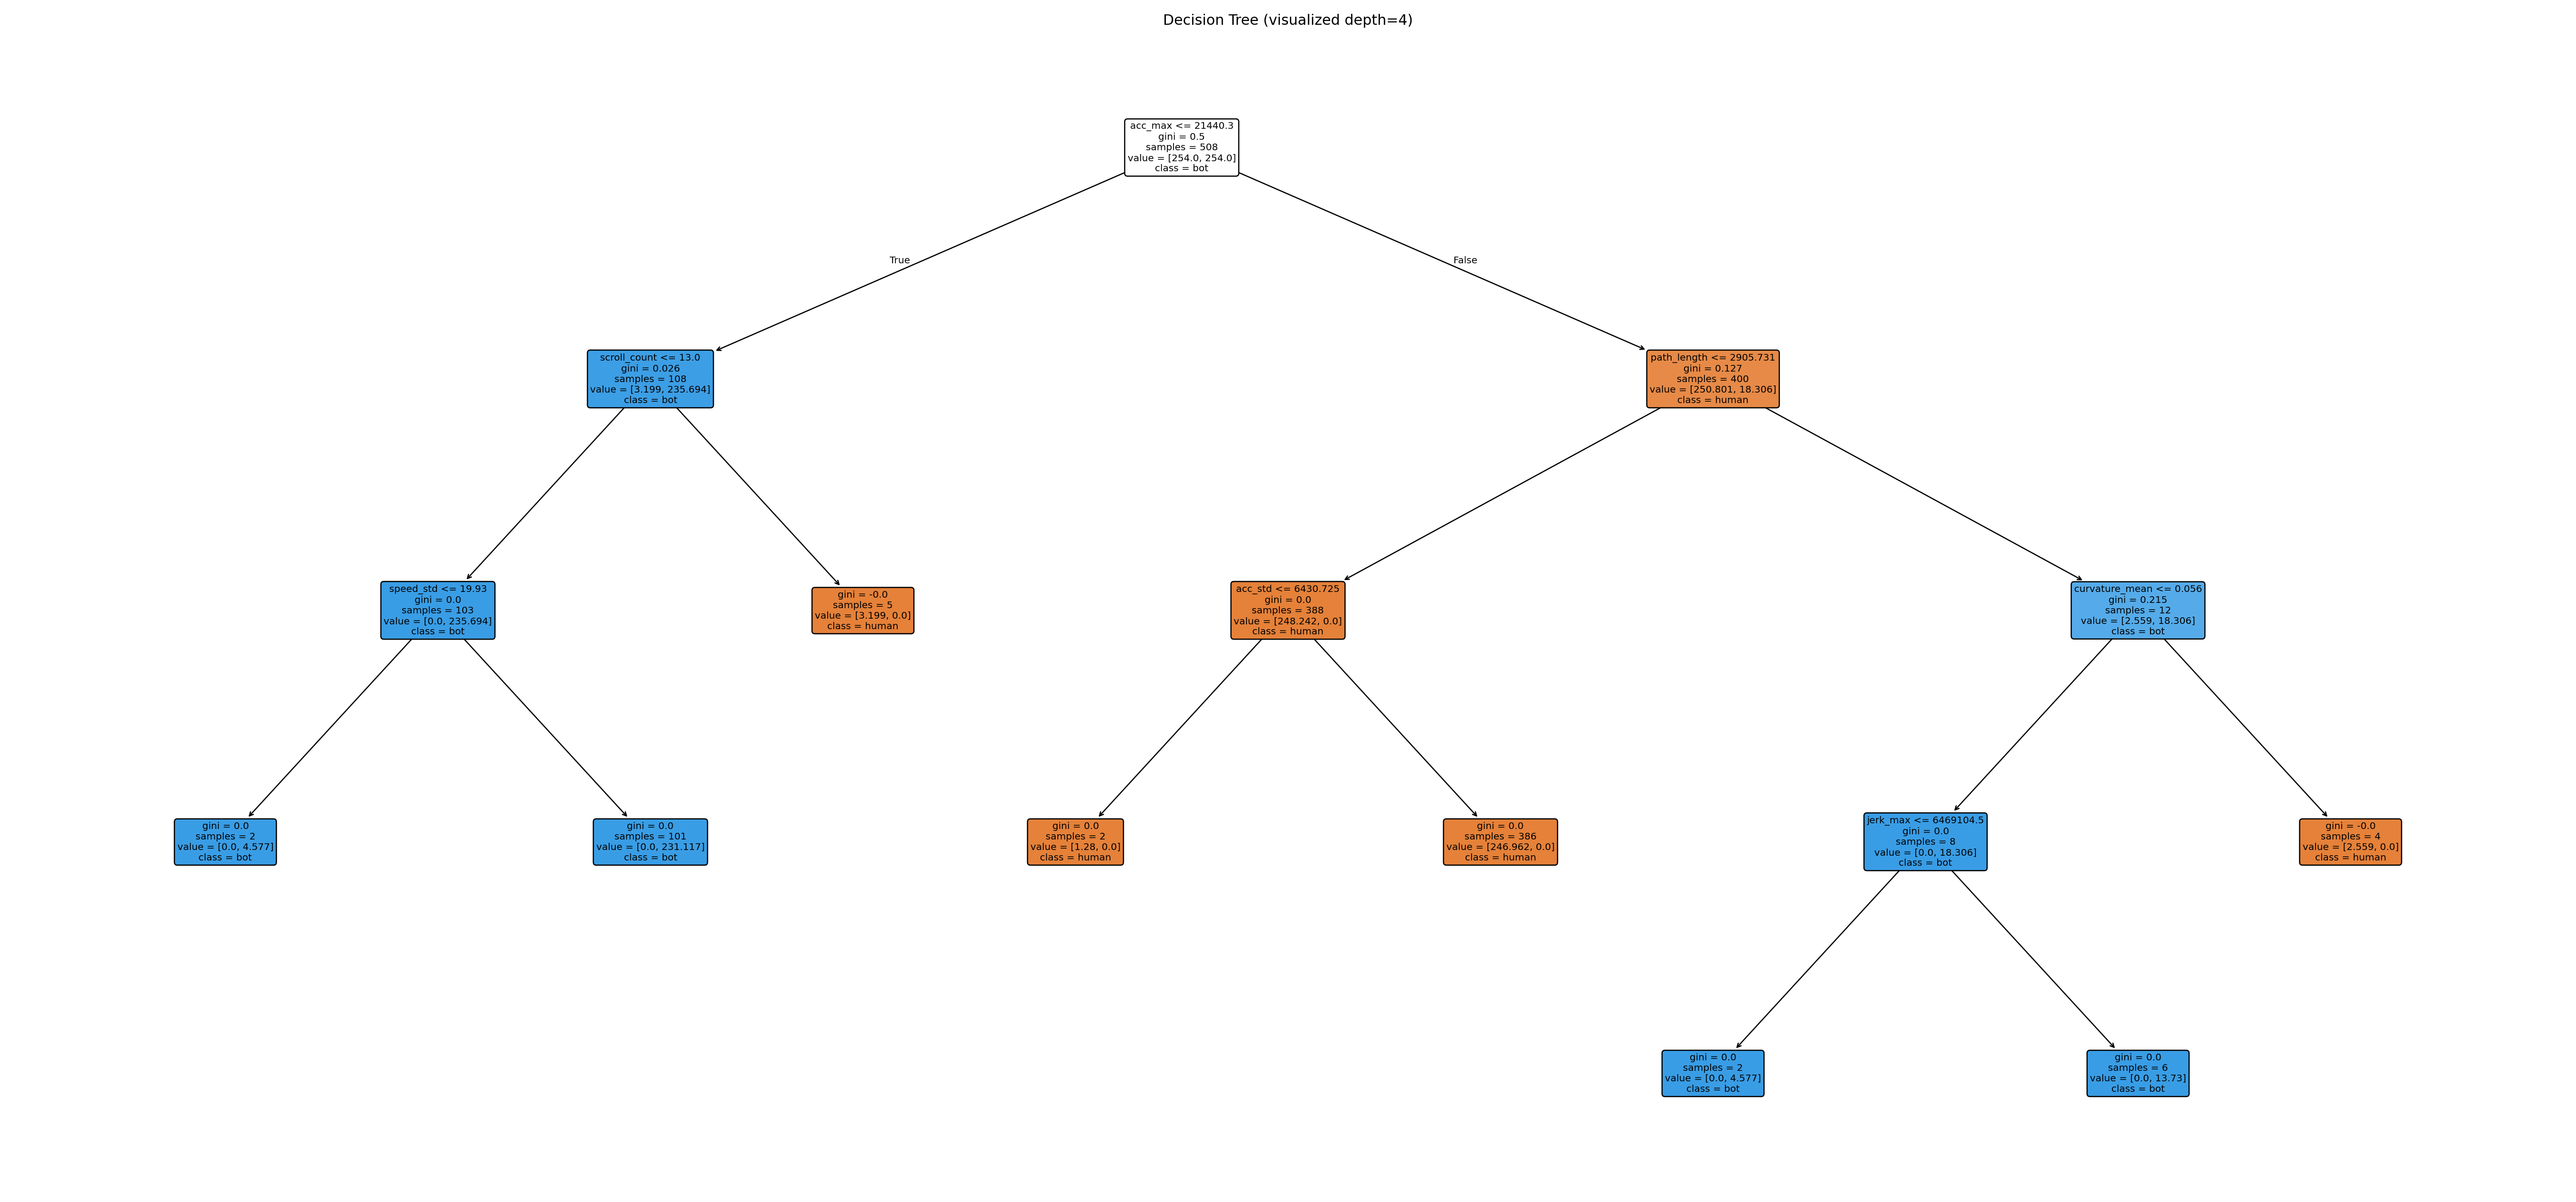
\includegraphics[width=0.72\textwidth]{figures/model/decision_tree_20260515_173306.png}
  \caption{Diagram drzewa decyzyjnego (warstwy najwyzszego poziomu)}
  \label{fig:model-tree}
\end{figure}

\begin{figure}[H]
  \centering
  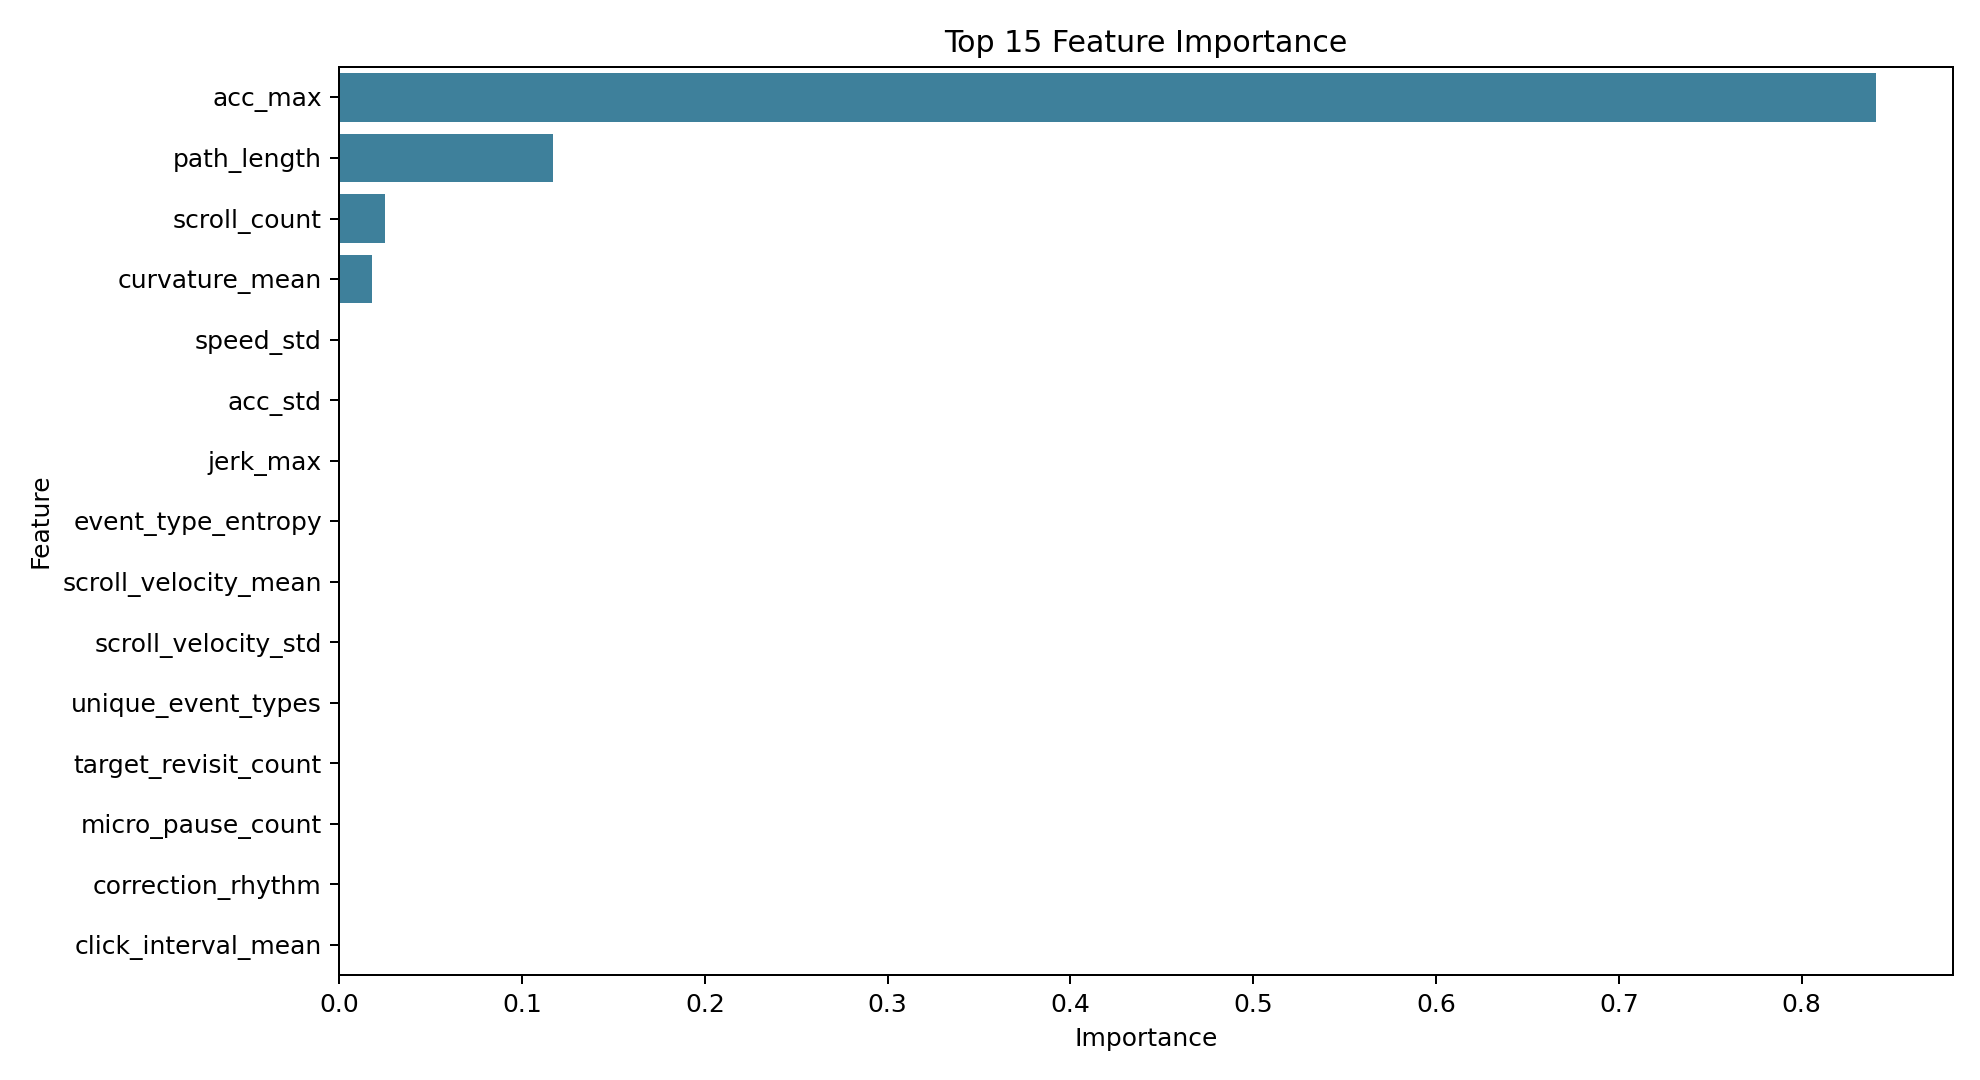
\includegraphics[width=0.8\textwidth]{figures/model/decision_tree_feature_importance_20260515_173306.png}
  \caption{Waznosc cech (feature importance) dla modelu finalnego}
  \label{fig:model-importance}
\end{figure}

\begin{figure}[H]
  \centering
  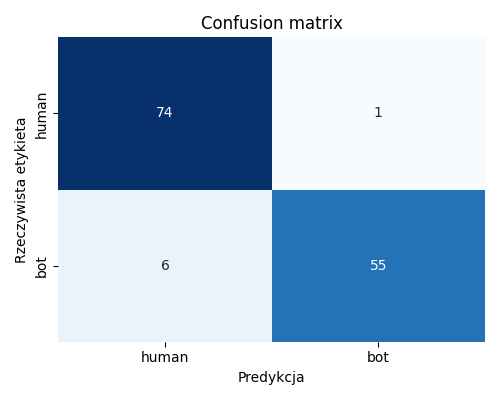
\includegraphics[width=0.45\textwidth]{figures/model/confusion_matrix_20260515_173306.png}
  \hfill
  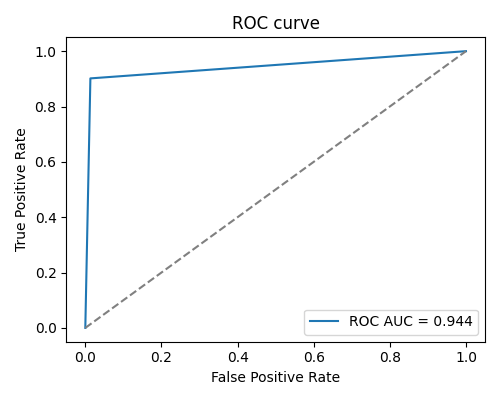
\includegraphics[width=0.45\textwidth]{figures/model/roc_20260515_173306.png}
  \caption{Confusion matrix oraz ROC dla zbioru testowego w treningu}
  \label{fig:train-cm-roc}
\end{figure}

\begin{figure}[H]
  \centering
  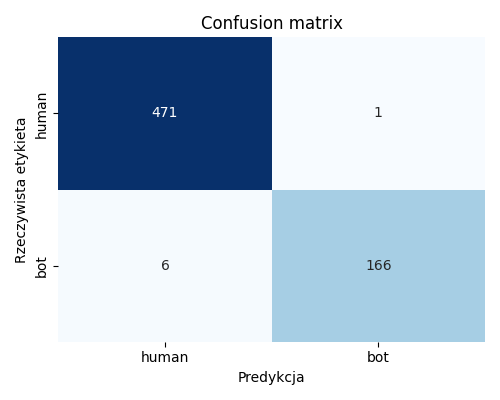
\includegraphics[width=0.45\textwidth]{figures/model/eval_confusion_matrix.png}
  \hfill
  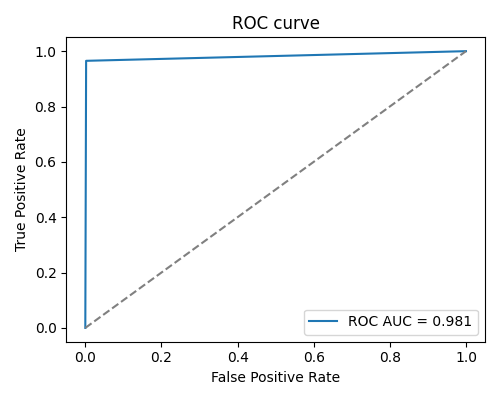
\includegraphics[width=0.45\textwidth]{figures/model/eval_roc.png}
  \caption{Confusion matrix oraz ROC w ewaluacji aktywnego modelu}
  \label{fig:eval-cm-roc}
\end{figure}

\subsection{Interpretacja: co model rzeczywiscie robi}
Rysunek~\ref{fig:model-tree} pokazuje, ze model jest interpretowalny i mozna
odczytac jawne warunki decyzji. Rysunek~\ref{fig:model-importance} potwierdza,
ze dominujaca cecha to nadal \texttt{acc\_max}, a kolejne sygnaly (np. \texttt{path\_length},
\texttt{event\_type\_entropy}) sa uzupelniajace.

\subsubsection{Struktura decyzyjna drzewa: interpretacja warstw}
Na podstawie Rysunku~\ref{fig:model-tree} i pelnych regul mozna odczytac
nastepujaca logike:
\begin{itemize}
  \item \textbf{Wezel glowny (\texttt{acc\_max})}: pierwszy podzial oddziela
  sesje o niskich i wysokich pikach przyspieszenia kursora.
  \item \textbf{Galaz niskiego \texttt{acc\_max}}: kolejne warunki
  \texttt{scroll\_count} i \texttt{speed\_std} prowadza glownie do klasy \texttt{bot}.
  Intuicyjnie: ruch jest bardziej wygladzony i mniej impulsywny.
  \item \textbf{Galaz wysokiego \texttt{acc\_max}}: podzialy po
  \texttt{path\_length} i \texttt{acc\_std} czesciej prowadza do klasy \texttt{human},
  bo odzwierciedlaja bardziej zrywny i korekcyjny tor ruchu.
  \item \textbf{Wezly glebsze} (\texttt{curvature\_mean}, \texttt{jerk\_max})
  doprecyzowuja decyzje dla przypadkow granicznych, gdzie sama dynamika pierwszego
  rzedu nie wystarcza.
\end{itemize}

\subsubsection{Jak czytac diagram waznosci cech}
Rysunek~\ref{fig:model-importance} przedstawia waznosci typu impurity-based
(spadek nieczystosci wezlow, Gini). Interpretacja:
\begin{itemize}
  \item wysoka waznosc \texttt{acc\_max} oznacza, ze ta cecha najczesciej daje
  najwiekszy przyrost informacji przy podzialach,
  \item niezerowa rola \texttt{path\_length} i \texttt{event\_type\_entropy}
  pokazuje, ze model korzysta takze z geometrii toru i roznorodnosci sekwencji eventow,
  \item niska waznosc wielu cech nie oznacza, ze sa globalnie niepotrzebne; oznacza,
  ze w aktualnej probie byly rzadziej wybierane jako najlepszy podzial.
\end{itemize}

\subsubsection{Znaczenie operacyjne (co to oznacza dla detekcji)}
Struktura drzewa jest spojna z celem systemu:
\begin{itemize}
  \item sesje o zbyt gladkiej mikrodynamice sa przesuwane w strone \texttt{bot},
  \item sesje z naturalnymi korektami i zrywami ruchu sa przesuwane w strone \texttt{human},
  \item policy engine otrzymuje wynik oparty o zachowanie, a nie o pojedynczy artefakt
  srodowiskowy.
\end{itemize}

\subsection{Reguly klasyfikacji (fragment)}
Model pozostaje interpretowalny -- mozna odczytac reguly decyzyjne:
\begin{lstlisting}[style=reportcode,caption={Przykladowy fragment regul drzewa decyzyjnego},label={lst:tree-rules-fragment}]
|--- acc_max <= 21440.2998
|   |--- scroll_count <= 13.0000
|   |   |--- speed_std <= 19.9304 -> class: bot
|--- acc_max > 21440.2998
|   |--- path_length <= 2905.7310
|   |   |--- acc_std > 6430.7249 -> class: human
\end{lstlisting}

Listing~\ref{lst:tree-rules-fragment} jest bezposrednim dopelnieniem
Rysunku~\ref{fig:model-tree}: po podziale na \texttt{acc\_max} drzewo
doprecyzowuje decyzje przez \texttt{scroll\_count}, \texttt{speed\_std},
\texttt{path\_length} i \texttt{acc\_std}. Taka sekwencja warunkow jest
czytelna biznesowo i latwa do audytu.

\subsection{Czy ewaluacja jest spojna z rzeczywistoscia?}
\subsubsection{Co jest spojne}
\begin{itemize}
  \item Hold-out test (Rysunek~\ref{fig:train-cm-roc}) i metryki z Tabeli~\ref{tab:train-metrics}
  pokazuja, ze model dobrze odroznia klasy na nieznanych sesjach testowych.
  \item Metryka \texttt{detection delay} (Tabela~\ref{tab:eval-operational}) daje praktyczny sygnal,
  po ilu eventach system zwykle wykrywa bota.
\end{itemize}

\subsubsection{Gdzie jest ryzyko przeszacowania}
\begin{itemize}
  \item Ewaluacja aktywnego modelu (Tabela~\ref{tab:eval-metrics}, Rysunek~\ref{fig:eval-cm-roc})
  liczona jest na calym zbiorze oznaczonych okien, wiec zawiera rowniez dane
  wykorzystane do treningu.
  \item To oznacza, ze wyniki ewaluacyjne sa bardziej optymistyczne niz hold-out
  i nie powinny byc jedynym kryterium oceny generalizacji.
\end{itemize}

\subsubsection{Najwazniejsze ograniczenie obecnego raportu}
W Tabeli~\ref{tab:eval-operational} \texttt{unseen\_bot\_recall} ma \texttt{count=0},
czyli w aktualnym zestawie nie ma osobnej, niewidzianej rodziny botow do twardego testu OOD.
Dlatego aktualny raport dobrze opisuje zachowanie modelu \emph{w ramach obecnej dystrybucji},
ale nie zamyka tematu odpornosci na nowe klasy botow.

\subsection{Threats to validity}
Ponizej wskazano glowne ryzyka interpretacyjne wynikow:
\begin{itemize}
  \item \textbf{Internal validity}: mimo wykluczenia czesci cech srodowiskowych z podzialow drzewa,
  pozostaje ryzyko, ze model wykorzystuje sygnaly specyficzne dla aktualnego UI i sposobu testowania.
  \item \textbf{Construct validity}: etykieta \texttt{human} opiera sie na recznym oznaczaniu sesji,
  co jest praktyczne, ale moze zawierac szum (np. sesja czlowieka z nienaturalnym rytmem).
  \item \textbf{External validity}: dane pochodza glownie z lokalnego srodowiska (localhost),
  ograniczonej liczby urzadzen/przegladarek i kontrolowanych scenariuszy.
  \item \textbf{Conclusion validity}: zastosowano pojedynczy hold-out split grupowy,
  bez wielokrotnej walidacji (\texttt{GroupKFold}) i bez przedzialow ufnosci metryk.
  \item \textbf{OOD validity}: brak niezaleznej rodziny botow w metryce \texttt{unseen\_bot\_recall}
  (\texttt{count=0}) utrudnia twarda ocene odpornosci na nowe techniki automatyzacji.
\end{itemize}

Wniosek praktyczny: metryki sa mocne dla aktualnej dystrybucji danych,
ale produkcyjna pewnosc wymaga dalszego rozszerzania zbioru i walidacji wielokrotnej.

\subsection{Wniosek koncowy}
Model finalny jest mocny i interpretowalny na aktualnym zbiorze (patrz
Tabela~\ref{tab:train-metrics} i Rysunek~\ref{fig:model-tree}),
jednak dla pelnej zgodnosci z warunkami produkcyjnymi potrzebuje kolejnego kroku:
oddzielnego testu na niewidzianych scenariuszach botowych oraz walidacji wielokrotnej
na poziomie sesji.


\section{Podsumowanie projektu}

\subsection{Co zostało osiągnięte}
W ramach MVP dostarczono działający system \textit{end-to-end}, który:
\begin{itemize}
  \item zbiera zachowania użytkownika w aplikacji webowej,
  \item buduje cechy behawioralne z krótkich okien czasowych,
  \item klasyfikuje sesje \texttt{human} vs \texttt{bot},
  \item generuje decyzję enforcement na podstawie \texttt{risk\_score},
  \item umożliwia trenowanie i ewaluację modelu na danych lokalnych.
\end{itemize}

\subsection{Wnioski praktyczne}
\begin{itemize}
  \item Podejście behawioralne daje dobrą wykrywalność nawet przy botach imitujących człowieka.
  \item Interpretowalne drzewo decyzyjne ułatwia prezentację i audyt decyzji modelu.
  \item Największy wpływ nadal mają cechy dynamiki ruchu (zwłaszcza \texttt{acc\_max}),
  więc doskonalenie botów powinno iść w stronę realistycznego modelowania nagłych zmian tempa.
\end{itemize}

\subsection{Rekomendowane kolejne kroki}
\begin{enumerate}
  \item Rozszerzyć zbiór o nowe rodziny botów i sesje \textit{unseen}.
  \item Dodać walidację czasową (time-based split) oraz monitoring driftu cech.
  \item Uzupełnić policy engine o reputację źródeł i denylistę.
  \item Rozważyć model sekwencyjny (np. Transformer/RNN) jako warstwę drugą.
  \item Dodać dashboard operacyjny do przeglądu sesji i interpretacji predykcji.
\end{enumerate}


\end{document}
